\documentclass[12pt]{article}
 
\usepackage[margin=1in]{geometry} 
\usepackage{amsmath,amsthm,amssymb,outlines}
\usepackage{graphicx}
\usepackage{tikzsymbols}
\newenvironment{statement}[2][Statement]{\begin{trivlist}
\item[\hskip \labelsep {\bfseries #1}\hskip \labelsep {\bfseries #2.}]}{\end{trivlist}}

\begin{document}
 
\title{MATH 8150 Homework 2} 
\author{Dahlen Elstran} 
\maketitle

\begin{statement}[Problem]{1}
  Prove that 
  \begin{align*}
    \int^{\infty}_0 \sin(x^2)dx=\int^{\infty}_0 \cos(x^2)dx=\frac{\sqrt{2\pi}}{4}.
  \end{align*}
\end{statement}
\begin{proof}
  First note that 
  \begin{align*}
    \int^{\infty}_0 e^{ix^2} = \int^{\infty}_0 \cos(x^2) dx + i \int^{\infty}_0 \sin(x^2)dx.
  \end{align*}
  Then by the hint, we know that
\end{proof}

\begin{statement}[Problem]{2}
  Show that 
  \begin{align*}
    \int^{\infty}_0 \frac{\sin(x)}{x} dx=\frac{\pi}{2}.
  \end{align*}
\end{statement}
\begin{proof}
  First, consider the following function $f(z)=\frac{e^{iz}}{z}$ and contour $\gamma$:
    \begin{center} 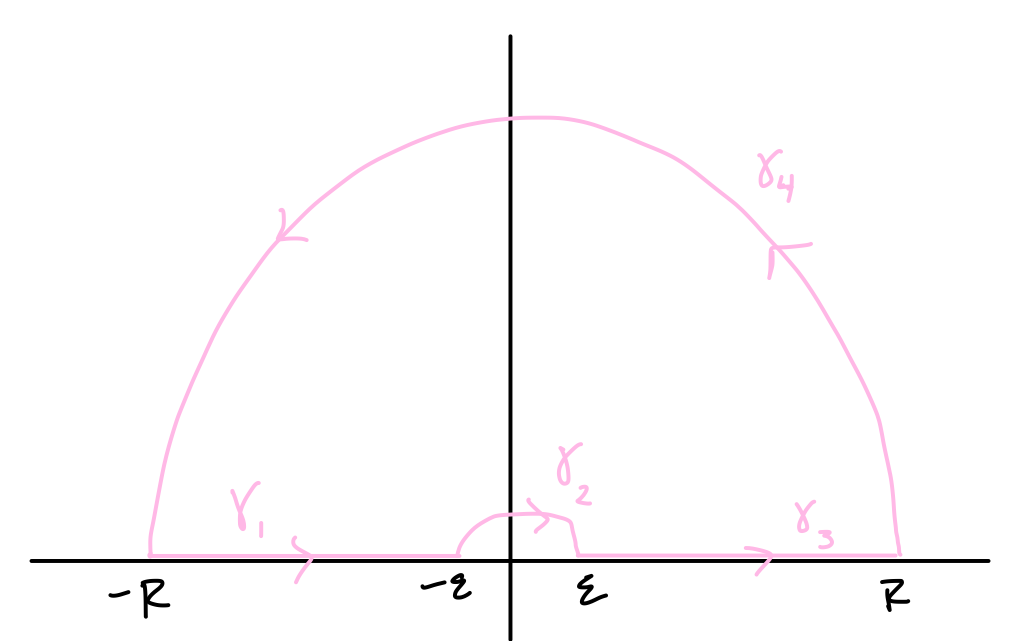
\includegraphics[scale=.2]{2-1.png} \end{center}
  Because the function is holomorphic on the closed contour, we can apply Cauchy's theorem to find that 
  \begin{equation*}
    \oint_{\gamma} f(z)dz = \int_{\gamma_1} f(z)dz + \int_{\gamma_2} f(z)dz + \int_{\gamma_3} f(z)dz +\int_{\gamma_4} f(z)dz = 0.
  \end{equation*}
  First, we evaluate the integrals over real numbers:
  \begin{equation*}
    \int_{\gamma_1} f(z)dz + \int_{\gamma_3} f(z)dz = \int_{-R}^{-\varepsilon} f(z)dz + \int_{\varepsilon}^{R} f(z)dz
  \end{equation*}
  Using u-subsitution and switch variables, we get 
  \begin{align*}
    \int^R_{\varepsilon} \frac{e^{ix}}{x}dx - \int^R_{\varepsilon} \frac{e^{-ix}}{x}dx &= \int^R_{\varepsilon} \frac{e^{ix}-e^{-ix}}{x}dx \\
                                                                                       &= 2i \int^R_{\varepsilon} \frac{e^{ix}-e^{-ix}}{(2i)x}dx \\
                                                                                       &= 2i \int^R_{\varepsilon} \frac{\sin (x)}{x}dx \\
                                                                                       & \to 2i \int^{\infty}_0 \frac{\sin (x)}{x}dx \text{ as } R \to \infty \text{ and } \varepsilon \to 0.
  \end{align*}
  Next, we evaluate the $\gamma_2$ integral with the following parametrization: 
  \begin{align*}
    z &=\gamma (t)= \varepsilon e^{i(\pi - t)} \text{ where } t \in [0,\pi]\\
    dz &= \gamma '(t)dt \\ 
       &= -i \varepsilon e^{i(\pi - t)} dt \\
       &= -i \gamma (t) dt
  \end{align*}
  So then
  \begin{align*}
  \int_{\gamma_2} \frac{e^{iz}}{z}dz &= \int^{\pi}_0 \frac{e^{i \gamma (t)}}{\gamma (t)}dt \\
                                     &= -i \int^{\pi}_0 e^{i \gamma (t)}dt \\
                                     &= -i \int^{\pi}_0 e^{i \varepsilon e^{i (\pi - t)}}dt
  \end{align*}
  As $\varepsilon \to 0$, this approaches 
  \begin{equation*}
    -i \int^{\pi}_0 1 \cdot dt = -i \pi.
  \end{equation*}
  For the last integral, use the following parametrization:
  \begin{align*}
    z &= \gamma(t)=Re^{it} \\
    dz &= \gamma ' (t)dt \\
       &= Re^{it}dt \\
       &= \gamma (t) dt
  \end{align*}
  So we have 
  \begin{align*}
    \int_{\gamma_4} f(z)dz &= \int^{\pi}_0 \frac{e^{i \gamma (t)}}{\gamma (t)} \gamma (t) dt \\
                           &= \int^{\pi}_0 e^{i \gamma (t)} dt \\
                           &= \int^{\pi}_0 e^{iRe^{it}} dt \\
                           &= \int^{\pi}_0 e^{iR(\cos (t) + i \sin (t))}dt. 
  \end{align*}
  Then note that 
  \begin{align*}
    \left\lvert \int^{\pi}_0 e^{iR(\cos (t) + i \sin (t))}dt \right\rvert & \leq \int^{\pi}_0 \left\lvert e^{iR(\cos (t) + i \sin (t))} \right \rvert dt \\
                                                                        &= \int^{\pi}_0 \left \lvert e^{iR\cos(t)} \right\rvert \left\lvert e^{-R\sin(t)}\right\rvert dt \\
                                                                        &= \int^{\pi}_0 1 \cdot \left\lvert e^{-R\sin(t)} \right\rvert dt \\
                                                                        &= \int^{\pi}_0 e^{-R\sin(t)}dt \\
                                                                        & \to 0 \text{ as } R \to \infty .
  \end{align*}
  So we find that this integral must be 0.
  Finally, we have 
  \begin{align*} 
    \oint_{\gamma} f(z)dz &= \int_{\gamma_1} f(z)dz + \int_{\gamma_2} f(z)dz + \int_{\gamma_3} f(z)dz +\int_{\gamma_4} f(z)dz \\
                          &= 2i \int^{\pi}_0 \frac{\sin(x)}{x} dx - i\pi + 0 \\
                          &= 0.
  \end{align*}
  Thus, 
  \begin{equation*}
    \int^{\pi}_0 \frac{\sin(x)}{x} dx = \frac{\pi}{2}.
  \end{equation*}
\end{proof}

\begin{statement}[Problem]{1}

\end{statement}
\begin{proof}

\end{proof}

\begin{statement}[Problem]{1}

\end{statement}
\begin{proof}

\end{proof}

\begin{statement}[Problem]{1}

\end{statement}
\begin{proof}

\end{proof}


\begin{statement}[Problem]{1}

\end{statement}
\begin{proof}

\end{proof}

\begin{statement}[Problem]{1}

\end{statement}
\begin{proof}

\end{proof}

\begin{statement}[Problem]{1}

\end{statement}
\begin{proof}

\end{proof}

\begin{statement}[Problem]{1}

\end{statement}
\begin{proof}

\end{proof}

\begin{statement}[Problem]{1}

\end{statement}
\begin{proof}

\end{proof}

\begin{statement}[Problem]{1}

\end{statement}
\begin{proof}

\end{proof}

\begin{statement}[Problem]{1}

\end{statement}
\begin{proof}

\end{proof}

\begin{statement}[Problem]{1}

\end{statement}
\begin{proof}

\end{proof}

\begin{statement}[Problem]{1}

\end{statement}
\begin{proof}

\end{proof}

\begin{statement}[Problem]{1}

\end{statement}
\begin{proof}

\end{proof}

\begin{statement}[Problem]{1}

\end{statement}
\begin{proof}

\end{proof}

\begin{statement}[Problem]{1}

\end{statement}
\begin{proof}

\end{proof}

\begin{statement}[Problem]{1}

\end{statement}
\begin{proof}

\end{proof}

\begin{statement}[Problem]{1}

\end{statement}
\begin{proof}

\end{proof}

\begin{statement}[Problem]{1}

\end{statement}
\begin{proof}

\end{proof}

\begin{statement}[Problem]{1}

\end{statement}
\begin{proof}

\end{proof}

\begin{statement}[Problem]{1}

\end{statement}
\begin{proof}

\end{proof}

\begin{statement}[Problem]{1}

\end{statement}
\begin{proof}

\end{proof}

\begin{statement}[Problem]{1}

\end{statement}
\begin{proof}

\end{proof}

\begin{statement}[Problem]{1}

\end{statement}
\begin{proof}

\end{proof}

\begin{statement}[Problem]{1}

\end{statement}
\begin{proof}

\end{proof}

\end{document}
